%================1.4
\section{Bộ phân tách tuyến tính theo tiếp cận của Fisher (Fisher's Linear discriminant Analysis - Fisher's LDA)}

Trong các bài toán phân loại mẫu thống kê, đối tượng quan sát thường được biểu diễn dưới dạng một vectơ đặc trưng nhiều chiều $\bm{x} \in \mathbb{R}^d$. Mỗi quan sát thuộc về một trong $K$ lớp $\{c_1,c_2,\ldots,c_K\}$ và mục tiêu của bài toán là xây dựng một quy tắc quyết định để từ một quan trắc mới có thể xác định phân lớp của nó một cách chính xác nhất có thể. Khi số chiều của dữ liệu lớn, việc phân loại trực tiếp trong không gian gốc thường gặp nhiều khó khăn do cấu trúc dữ liệu phức tạp, khả năng trực quan hóa hạn chế, và nguy cơ tồn tại những biến không thật sự hữu ích cho việc phân biệt lớp.

\hspace*{0.5cm}Phân tích tách biệt tuyến tính (Linear Discriminant Analysis -- LDA) là một trong những phương pháp kinh điển của thống kê nhiều chiều cho cả hai mục tiêu: \emph{giảm chiều có giám sát} và \emph{phân loại}. Điều đáng chú ý là LDA có thể được hiểu từ hai góc nhìn khác nhau nhưng thống nhất ở kết quả cuối cùng. Góc nhìn thứ nhất là cách tiếp cận của Fisher, trong đó ta tìm một phép chiếu tuyến tính sao cho dữ liệu sau khi chiếu tách biệt lớp tốt nhất. Góc nhìn thứ hai là lý thuyết quyết định Bayes, trong đó quy tắc phân loại tối ưu được xây dựng từ xác suất hậu nghiệm; dưới giả thiết Gaussian với cùng ma trận hiệp phương sai, quy tắc Bayes dẫn đến một bộ phân loại tuyến tính. Chính sự gặp nhau của hai hướng tiếp cận này tạo nên nền tảng lý thuyết hoàn chỉnh của LDA.

\hspace*{0.5cm}Vì vậy, để hiểu đầy đủ phương pháp LDA, chương này sẽ trình bày lần lượt ba nội dung chính. Trước hết là cách tiếp cận của Fisher với tiêu chuẩn tối đa hóa sự tách biệt giữa các lớp. Tiếp theo là cơ sở của lý thuyết quyết định Bayes trong bài toán phân loại. Cuối cùng, trên nền tảng Bayes, ta chỉ ra cách mô hình Gaussian với ma trận hiệp phương sai chung sẽ dẫn trực tiếp đến LDA, đồng thời cho thấy sự tương đương giữa hai cách tiếp cận trên.

%================1.4.1
\subsection{Ý tưởng hình học của Fisher}

Khác với lý thuyết Bayes, Fisher xuất phát từ một câu hỏi mang tính hình học: nếu dữ liệu đã có nhãn lớp, có thể tìm được một phép chiếu tuyến tính sao cho sau khi chiếu, các lớp được tách biệt tốt nhất hay không? Trong trường hợp hai lớp, Fisher tìm một vectơ $\bm{\beta}$ (có độ dài đơn vị) để chiếu dữ liệu từ không gian $\mathbb{R}^d$ xuống không gian con sinh bởi vectơ $\bm{\beta}$.

Sau phép chiếu này, mỗi lớp sẽ có một trung bình và một mức độ phân tán riêng. Một hướng chiếu tốt là hướng làm khoảng cách giữa các trung bình lớp trên trục chiếu càng lớn càng tốt, đồng thời làm phương sai trong từng lớp trên trục chiếu càng nhỏ càng tốt.

Giả sử bài toán gồm hai lớp \(C_1\) và \(C_2\). Mỗi quan sát được biểu diễn bởi một vectơ \(\bm{x}\in\mathbb{R}^d\). Fisher tìm một hướng chiếu sao cho sau khi chiếu dữ liệu xuống một trục, hai lớp cách xa nhau nhất hoặc ít chồng lấn nhất.

\begin{figure}[H]
	\centering
	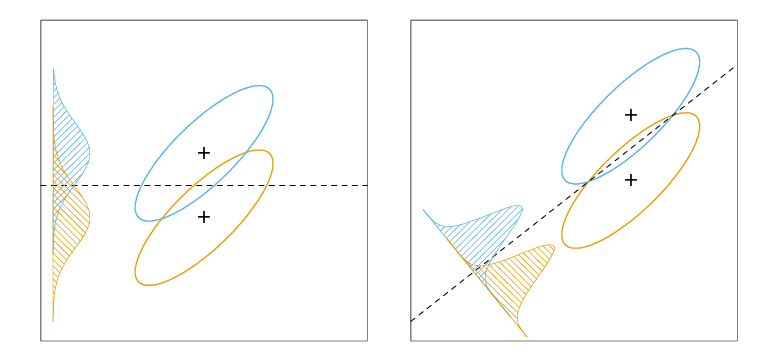
\includegraphics[width=0.8\textwidth]{image/image_1_Fisher_idea.png}
	\caption{Ý tưởng hình học của Fisher để phân tách hai lớp tốt nhất, xem tài liệu \cite{hastie2009}.}
	\label{fig:hinh1}
\end{figure}
Để lượng hóa hai ý tưởng ``cách xa nhau nhất giữa các lớp'' và ``tụ lại ở trong lớp'', Fisher đưa vào hai đại lượng cơ bản.
Gọi $\bm{\mu}$ là trung bình mẫu của toàn bộ dữ liệu. Ma trận tán xạ giữa các lớp được xác định bởi
\begin{equation}
	\Sigma_B = \sum_{k=1}^{K} n_k(\bm{\mu}_k-\bm{\mu})(\bm{\mu}_k-\bm{\mu})^T,
\end{equation}
trong đó,
\[
\bm{\mu}_k
=
\frac{1}{n_k}
\sum_{\bm{x}_i \in C_k}
\bm{x}_i,
\qquad k=1,2.
\]
là vectơ trung bình mẫu của từng lớp;
\[
\bm{\mu}
=
\frac{1}{n}
\sum_{i=1}^{n}
\bm{x}_i
\]
là vectơ trung bình mẫu của toàn bộ dữ liệu mẫu. Ma trận này phản ánh mức độ phân tách giữa các lớp thông qua vị trí tương đối của các trung bình lớp so với trung bình toàn cục.

Với mỗi lớp $C_{k}$, gọi $\bm{\mu}_k$ là vectơ trung bình mẫu của lớp đó. Ma trận tán xạ trong lớp được xác định bởi
\begin{equation}
\Sigma_W
=
\sum_{k=1}^{K}
\sum_{\bm{x}_i \in C_k}
(\bm{x}_i-\bm{\mu}_k)(\bm{x}_i-\bm{\mu}_k)^T.
\end{equation}
Ma trận này mô tả độ phân tán của các điểm quanh trung bình lớp tương ứng. Nếu các điểm trong từng lớp tập trung lại gần nhau thì $\Sigma_W$ nhỏ; ngược lại, nếu dữ liệu phân tán rộng thì $\Sigma_W$ lớn.

Trong trường hợp hai lớp, Fisher xét biến chiếu $z = \bm{\beta}^T \bm{x}$. Gọi $m_1 = \bm{\beta}^T \bm{\mu}_1$ và $m_2 = \bm{\beta}^T \bm{\mu}_2$ là trung bình của hai lớp sau chiếu. Khi đó, độ tách biệt giữa hai lớp trên phương chiếu có thể đo bằng $(m_1-m_2)^2$. Đồng thời, phương sai trong lớp sau chiếu là
\begin{equation}
\sigma_W^2 = \bm{\beta}^T \Sigma_W \bm{\beta}.
\end{equation}
Do đó, tiêu chuẩn Fisher được viết thành
\begin{equation}
J(\bm{\beta})
=
\frac{(\bm{\beta}^T(\bm{\mu}_1-\bm{\mu}_2))^2}{\bm{\beta}^T \Sigma_W \bm{\beta}}
=
\frac{\bm{\beta}^T \Sigma_B \bm{\beta}}{\bm{\beta}^T \Sigma_W \bm{\beta}}.
\end{equation}
Mục tiêu là tìm $\bm{\beta} \neq 0$ sao cho $J(\bm{\beta})$ đạt cực đại.

\subsection{Nghiệm tối ưu của Fisher trong trường hợp hai lớp}
Gọi $\bm{\mu}_1,\bm{\mu}_2$ lần lượt là vectơ trung bình của hai lớp. Khi đó, ma trận tán xạ giữa hai lớp được xác định bởi
\[
\Sigma_B
=
(\bm{\mu}_1-\bm{\mu}_2)(\bm{\mu}_1-\bm{\mu}_2)^T.
\]
Ma trận tán xạ trong lớp (ma trận phương sai mẫu gộp - pooled variance matrix) được xác định bởi
\[
\Sigma_W
=
\frac{(n_1-1)\Sigma_1+(n_2-1)\Sigma_2}{n-2},
\]
trong đó $n=n_1+n_2$, còn $\Sigma_1,\Sigma_2$ lần lượt là ma trận hiệp phương sai mẫu của hai lớp
\[
\Sigma_1
=
\frac{1}{n_1-1}
\sum_{i=1}^{n_1}
(\bm{x}_{i1}-\bm{\mu}_1)(\bm{x}_{i1}-\bm{\mu}_1)^T,
\]

\[
\Sigma_2
=
\frac{1}{n_2-1}
\sum_{i=1}^{n_2}
(\bm{x}_{i2}-\bm{\mu}_2)(\bm{x}_{i2}-\bm{\mu}_2)^T.
\]
Tiêu chuẩn Fisher được viết dưới dạng
\[
J(\bm{\beta})
=
\frac{\bm{\beta}^T\Sigma_B\bm{\beta}}
{\bm{\beta}^T\Sigma_W\bm{\beta}},
\qquad
\bm{\beta}\in\mathbb{R}^d.
\]

Mục tiêu là tìm vectơ chiếu $\bm{\beta}$ sao cho $J(\bm{\beta})$  đạt giá trị lớn nhất
\[
\max_{\bm{\beta}\neq \bm{0}}
J(\bm{\beta})
=
\max_{\bm{\beta}\neq \bm{0}}
\frac{\bm{\beta}^T\Sigma_B\bm{\beta}}
{\bm{\beta}^T\Sigma_W\bm{\beta}}.
\]
Vì $\Sigma_W$ là ma trận đối xứng xác định dương nên tồn tại phân rã phổ
\[
\Sigma_W
=
D\Lambda D^T,
\]
trong đó $D$ là ma trận trực giao chứa các vectơ riêng của $\Sigma_W$, còn $\Lambda$ là ma trận đường chéo chứa các giá trị riêng dương thỏa
\[
D^TD=I,
\qquad
\Lambda
=
\operatorname{diag}(\lambda_1,\lambda_2,\ldots,\lambda_d),
\]
với
\[
\lambda_1,\lambda_2,\ldots,\lambda_d>0.
\]

Do đó, ta đặt
\[
\Sigma_W^{1/2}
=
D\Lambda^{1/2}D^T,
\]
trong đó,
\[
\Lambda^{1/2}
=
\operatorname{diag}
\left(
\sqrt{\lambda_1},
\sqrt{\lambda_2},
\ldots,
\sqrt{\lambda_d}
\right).
\]

Tương tự, ta đặt
\[
\Sigma_W^{-1/2}
=
D\Lambda^{-1/2}D^T,
\]
với,
\[
\Lambda^{-1/2}
=
\operatorname{diag}
\left(
\frac{1}{\sqrt{\lambda_1}},
\frac{1}{\sqrt{\lambda_2}},
\ldots,
\frac{1}{\sqrt{\lambda_d}}
\right).
\]

Lúc này, với
\[
\bm{y}
=
\Sigma_W^{1/2}\bm{\beta},
\]
ta suy ra,
\[
\bm{\beta}
=
\Sigma_W^{-1/2}\bm{y}.
\tag{*}
\label{*}
\]

Thay vào tiêu chuẩn Fisher, ta được
\[
J(\bm{\beta})
=
\frac{\bm{\beta}^T \Sigma_B \bm{\beta}}
{\bm{\beta}^T \Sigma_W \bm{\beta}}
=
\frac{\bm{y}^T S \bm{y}}{\bm{y}^T \bm{y}}.
\]

Thực vậy, xét mẫu số trước
\[
\bm{\beta}^T\Sigma_W\bm{\beta}
=
\left(\Sigma_W^{-1/2}\bm{y}\right)^T
\Sigma_W
\left(\Sigma_W^{-1/2}\bm{y}\right).
\]
Vì $\Sigma_W^{-1/2}$ đối xứng nên
\[
\bm{\beta}^T\Sigma_W\bm{\beta}
=
\bm{y}^T
\Sigma_W^{-1/2}
\Sigma_W
\Sigma_W^{-1/2}
\bm{y}.
\]
Mà
\[
\begin{aligned}
	\Sigma_W^{-1/2}
	\Sigma_W
	\Sigma_W^{-1/2}
	&=
	D\Lambda^{-1/2}D^T
	D\Lambda D^T
	D\Lambda^{-1/2}D^T \\[0.2cm]
	&=
	D\Lambda^{-1/2}
	(D^TD)
	\Lambda
	(D^TD)
	\Lambda^{-1/2}D^T \\[0.2cm]
	&=
	D\Lambda^{-1/2}
	\Lambda
	\Lambda^{-1/2}D^T \\[0.2cm]
	&=
	DD^T \\[0.2cm]
	&=
	I.
\end{aligned}
\]
nên,
\[
\bm{\beta}^T\Sigma_W\bm{\beta}
=
\bm{y}^T\bm{y}.
\]

Tương tự, tử số trở thành
\[
\bm{\beta}^T\Sigma_B\bm{\beta}
=
\left(\Sigma_W^{-1/2}\bm{y}\right)^T
\Sigma_B
\left(\Sigma_W^{-1/2}\bm{y}\right).
\]
Do đó,
\[
\bm{\beta}^T\Sigma_B\bm{\beta}
=
\bm{y}^T
\left(\Sigma_W^{-1/2}\right)^T
\Sigma_B
\Sigma_W^{-1/2}
\bm{y}.
\]

Vì $\Sigma_W^{-1/2}$ đối xứng nên
\[
\left(\Sigma_W^{-1/2}\right)^T
=
\Sigma_W^{-1/2}.
\]
Đặt,
\[
S
=
\left(\Sigma_W^{-1/2}\right)^T
\Sigma_B
\Sigma_W^{-1/2}
=
\Sigma_W^{-1/2}
\Sigma_B
\Sigma_W^{-1/2}.
\]

Khi đó, tiêu chuẩn Fisher trở thành
\[
J(\bm{\beta})
=
\frac{\bm{y}^T S \bm{y}}{\bm{y}^T\bm{y}}.
\]
Vì $\Sigma_B$ đối xứng và $\Sigma_W^{-1/2}$ đối xứng nên $S$ cũng là ma trận đối xứng
\[
S^T=S.
\]
Do đó, bài toán tối ưu Fisher được đưa về bài toán
\[
\max_{\bm{y}\neq \bm{0}}
\frac{\bm{y}^T S \bm{y}}{\bm{y}^T\bm{y}}.
\]

Đây chính là bài toán thương Rayleigh.

Đặt,
\[
\bm{x}
=
\frac{\bm{y}}{\|\bm{y}\|},
\qquad
\|\bm{x}\|=1.
\]

Khi đó,
\[
\frac{\bm{y}^T S \bm{y}}{\bm{y}^T\bm{y}}
=
\bm{x}^T S \bm{x}.
\]

Vì $S$ là ma trận đối xứng xác định không âm nên tồn tại phân rã phổ
\[
S
=
U\Gamma U^T,
\]
trong đó,
\[
U^TU=I,
\]
và,
\[
\Gamma
=
\operatorname{diag}(\gamma_1,\gamma_2,\ldots,\gamma_d),
\quad \text{với} \quad
\gamma_1\geq \gamma_2\geq \cdots \geq \gamma_d \geq 0.
\]

Đặt,
\begin{equation}
	\bm{z}
	=
	U^T\bm{x}.
	\tag{**}
	\label{**}
\end{equation}

Ta có,
\[
\|\bm{z}\|^2
=
\bm{z}^T\bm{z}
=
\bm{x}^TUU^T\bm{x}
=
\bm{x}^T\bm{x}
=
1.
\]

Mặt khác,
\[
\bm{x}^T S \bm{x}
=
\bm{x}^T U\Gamma U^T\bm{x}
=
\bm{z}^T\Gamma \bm{z}.
\]

Suy ra,
\[
\bm{x}^T S \bm{x}
=
\gamma_1z_1^2
+
\gamma_2z_2^2
+
\cdots
+
\gamma_dz_d^2.
\]

Do,
\[
\gamma_1\geq \gamma_2\geq \cdots \geq \gamma_d,
\]
nên
\[
\bm{x}^T S \bm{x}
\leq
\gamma_1(z_1^2+z_2^2+\cdots+z_d^2).
\]

Mặt khác,
\[
z_1^2+z_2^2+\cdots+z_d^2
=
\|\bm{z}\|^2
=
1.
\]
nên
\[
\bm{x}^T S \bm{x}
\leq
\gamma_1.
\]

Dấu ``='' xảy ra khi và chỉ khi $\bm{z}_{\text{opt}}=(1,0,\ldots,0)^T$. Kết hợp với~\eqref{**}, ta có 
\[
\bm{x}_{\text{opt}}
=
U\bm{z}_{\text{opt}},
\]
là vectơ riêng ứng với giá trị riêng lớn nhất của $S$.

Hơn nữa, vì
\[
\bm{x}
=
\frac{\bm{y}}{\|\bm{y}\|},
\]
nên
\[
\bm{y}_{\text{opt}}
\propto
\bm{x}_{\text{opt}}.
\]

Kết hợp với~\eqref{*}, ta suy ra
\begin{equation}
	\bm{\beta}_{\text{opt}}
	\propto
	\Sigma_W^{-1/2}\bm{x}_{\text{opt}}.
	\tag{***}
	\label{***}
\end{equation}

Do $\bm{x}_{\text{opt}}$ là vectơ riêng ứng với giá trị riêng lớn nhất của $S$ nên
\[
S\bm{x}_{\text{opt}}
=
\gamma_1\bm{x}_{\text{opt}}
\quad \Longleftrightarrow \quad
\left(\Sigma_W^{-1/2}\right)^T
\Sigma_B
\left(\Sigma_W^{-1/2}\right)
\bm{x}_{\text{opt}}
=
\gamma_1\bm{x}_{\text{opt}}.
\]

Đặt, $
\bm{u}_{\text{opt}}
=
\Sigma_W^{-1/2}\bm{x}_{\text{opt}}
$, suy ra $\bm{\beta}_{\text{opt}}
\propto
\bm{u}_{\text{opt}}$ và $\bm{x}_{\text{opt}}
=
\Sigma_W^{1/2}\bm{u}_{\text{opt}}$
\[
\begin{aligned}
	\Sigma_W^{-1/2}\Sigma_B\Sigma_W^{-1/2}
	\bm{x}_{\text{opt}}
	&=
	\gamma_1\bm{x}_{\text{opt}} \\[0.2cm]
	\Sigma_W^{-1/2}\Sigma_B\Sigma_W^{-1/2}
	\Sigma_W^{1/2}\bm{u}_{\text{opt}}
	&=
	\gamma_1\Sigma_W^{1/2}\bm{u}_{\text{opt}} \\[0.2cm]
	\Sigma_W^{-1/2}\Sigma_B\bm{u}_{\text{opt}}
	&=
	\gamma_1\Sigma_W^{1/2}\bm{u}_{\text{opt}} \\[0.2cm]
	\Rightarrow \quad
	\Sigma_W^{-1}\Sigma_B\bm{u}_{\text{opt}}
	&=
	\gamma_1\bm{u}_{\text{opt}}.
\end{aligned}
\]

Lưu ý, do
\[
\Sigma_B
=
(\bm{\mu}_1-\bm{\mu}_2)(\bm{\mu}_1-\bm{\mu}_2)^T.
\]
nên
\[
\Sigma_W^{-1}
\Sigma_B
\bm{u}_{\text{opt}}
=
\Sigma_W^{-1}
(\bm{\mu}_1-\bm{\mu}_2)(\bm{\mu}_1-\bm{\mu}_2)^T
\bm{u}_{\text{opt}}.
\]

Đặt, $\bm{v}
=
\Sigma_W^{-1}(\bm{\mu}_1-\bm{\mu}_2)
\in \mathbb{R}^d,
\quad
\bm{w}
=
\bm{\mu}_1-\bm{\mu}_2$, khi đó
\[
\bm{v}\,
\underbrace{\bm{w}^T\bm{u}_{\text{opt}}}_{\in \mathbb{R}}
=
\underbrace{\bm{w}^T\bm{u}_{\text{opt}}}_{\in \mathbb{R}}\,
\bm{v}
=
\gamma_1
\bm{u}_{\text{opt}}.
\]

Suy ra $\bm{u}_{\text{opt}}
\propto
\Sigma_W^{-1}(\bm{\mu}_1-\bm{\mu}_2)$, hay
\[
\bm{\beta}_{\text{opt}}
\propto
\Sigma_W^{-1}(\bm{\mu}_1-\bm{\mu}_2).
\]

Một cách tiếp cận khác có thể sử dụng để tìm nghiệm tối ưu trên là sử dụng bất đẳng thức Cauchy--Schwarz cho tích vô hướng trong $\mathbb{R}^d$. Tuy nhiên, nội dung này sẽ không được trình bày trong phạm vi của đồ án.

Do tiêu chuẩn Fisher không thay đổi khi nhân $\bm{\beta}$ với một hằng số khác $0$, nên ta thường chọn
\[
\boxed{
	\bm{\beta}_{\text{opt}}
	=
	\Sigma_W^{-1}(\bm{\mu}_1-\bm{\mu}_2)
}
\]

Như vậy, trong trường hợp hai lớp, nghiệm tối ưu của Fisher là vectơ chiếu theo hướng nghịch đảo ma trận tán xạ trong lớp nhân với hiệu vectơ trung bình của hai lớp.

\hspace*{0.5cm}Sau khi đã xác định được phương chiếu tối ưu $\bm{\beta}_{\text{opt}}$, việc phân lớp một đối tượng có giá trị của vectơ các biến quan trắc $\bm{x}$ được thực hiện theo thủ tục sau

Với $\bm{X}=\bm{x} \in \mathbb{R}^d$, đặt $y=\bm{\beta}_{\text{opt}}^T\bm{x}$.
\[
\widehat{G}(\bm{x})
=
\arg\min_{k=1,2}
\left|y-\bar{y}_k\right|,
\]
với $\bar{y}_k=\bm{\beta}_{\text{opt}}^T\bm{\mu}_k,\ k=1,2$.

Như vậy, biên tách biệt tuyến tính của mô hình được cho bởi phương trình
\[
\left|y_{\text{bnd}}-\bar{y}_1\right|
=
\left|y_{\text{bnd}}-\bar{y}_2\right|
\]
hay
\begin{equation}
	2y_{\text{bnd}}-\left(y_1+y_2\right)=0.
	\label{eq:y-bnd}
\end{equation}

Thay $y_{\text{bnd}}=\bm{\beta}_{\text{opt}}^T\bm{x}_{\text{bnd}}$, $y_k=\bm{\beta}_{\text{opt}}^T\bm{\mu}_k \ (k=1,2)$ vào \eqref{eq:y-bnd}, với $\bm{\beta}_{\text{opt}}
=
\Sigma_W^{-1}(\bm{\mu}_1-\bm{\mu}_2)$ ta có
\[
\left[\Sigma_W^{-1}(\bm{\mu}_1-\bm{\mu}_2)\right]^T
\bm{x}_{\text{bnd}}
-
\frac{1}{2}
\left[
\bm{\mu}_1^T\Sigma_W^{-1}(\bm{\mu}_1-\bm{\mu}_2)
+
\bm{\mu}_2^T\Sigma_W^{-1}(\bm{\mu}_1-\bm{\mu}_2)
\right]
=
0
\]
\begin{equation}
	\quad \Longleftrightarrow \quad
	\left[\Sigma_W^{-1}(\bm{\mu}_1-\bm{\mu}_2)\right]^T
	\bm{x}_{\text{bnd}}
	-
	\frac{1}{2}
	\left(
	\bm{\mu}_1^T\Sigma_W^{-1}\bm{\mu}_1
	-
	\bm{\mu}_2^T\Sigma_W^{-1}\bm{\mu}_2
	\right)
	=
	0.
	\label{eq:class}
\end{equation}

























